\subsection{Transfer to a two-loop propagator family}
We also applied the unchanged interfaces to the massless two-loop
propagator family used in the earlier cost comparisons. Its five
independent family indices fit the compiled row interface. We fixed
two batches of 16 and 64 stored target expressions and all policies
before this transfer calculation. Each method uses five rotated
repetitions, the same master basis and the same time and memory limits.
Storage-interrupted trials resume on their original node, with earlier
observations preserved. Because this family appeared in earlier
comparisons, this experiment measures transfer of the revised
implementation and does not establish generalization to a newly unseen
family.

Alongside native seeding and the full candidate pool, we include a
deterministic source-row control using the same compiled reduction
structure. This control selects a source by row length and integral ordering
within the same changing leading-column group. Comparing the learned row policy
with this control separates the source choice from changes to the
compiled reduction structure. Every completed reduction receives the
same exact coefficient check and an independent finite-field check.

The transfer experiment contains 60 measured trials among 60 planned records, with 60 exact completions. The independent audit performed 7,200 target-coefficient checks and 2,355 row-update checks.

For 16 targets, the native control's median complete time was $12.003$ seconds. The learned seed filter gave a time ratio of $0.992$ with descriptive interval $[0.962,1.030]$; the learned source-row policy gave a time ratio of $0.991$ with descriptive interval $[0.984,1.022]$; the combined policy gave a time ratio of $0.976$ with descriptive interval $[0.961,0.996]$. In the matched controls, the learned seed filter relative to the full pool had ratio $1.051$ with interval $[1.024,1.072]$ and the learned source choice relative to the deterministic compiled control had ratio $0.987$ with interval $[0.979,1.034]$.

For 64 targets, the native control's median complete time was $12.770$ seconds. The learned seed filter gave a time ratio of $1.758$ with descriptive interval $[1.744,1.777]$; the learned source-row policy gave a time ratio of $0.976$ with descriptive interval $[0.964,0.992]$; the combined policy gave a time ratio of $1.755$ with descriptive interval $[1.740,1.777]$. In the matched controls, the learned seed filter relative to the full pool had ratio $1.907$ with interval $[1.880,1.920]$ and the learned source choice relative to the deterministic compiled control had ratio $0.987$ with interval $[0.952,1.012]$.


The compiled learned-row pipeline reduced the median complete time for
64 targets from 12.770 to 12.460 seconds, a measured reduction of
2.4\%. Its ratio against the deterministic compiled control has an
interval that includes one, so this experiment does not resolve a
benefit caused by the learned source choice itself. The full-pool
control was faster, at 11.773 seconds. For 16 targets, the combined
pipeline reduced the native median by 2.4\%, but the full-pool control
again completed sooner. For 64 targets, every learned-seed and combined
trial required fallback, whose cost is included in the reported time.
These observations establish limited gains relative to the stated
native baseline and also identify stronger deterministic controls.


Figure~\ref{fig:native-transfer} shows all complete paired comparisons.
A ratio below one denotes a lower median complete time. The intervals
come from 10,000 paired resamples of the five repetitions and describe
repeat-to-repeat variation within this one family. They do not measure
uncertainty across different integral families. Incomplete pairs remain
in the completion counts and receive no timing ratio
\cite{KiraNativeAccelerationData}.

\begin{figure}[htbp]
 \centering
 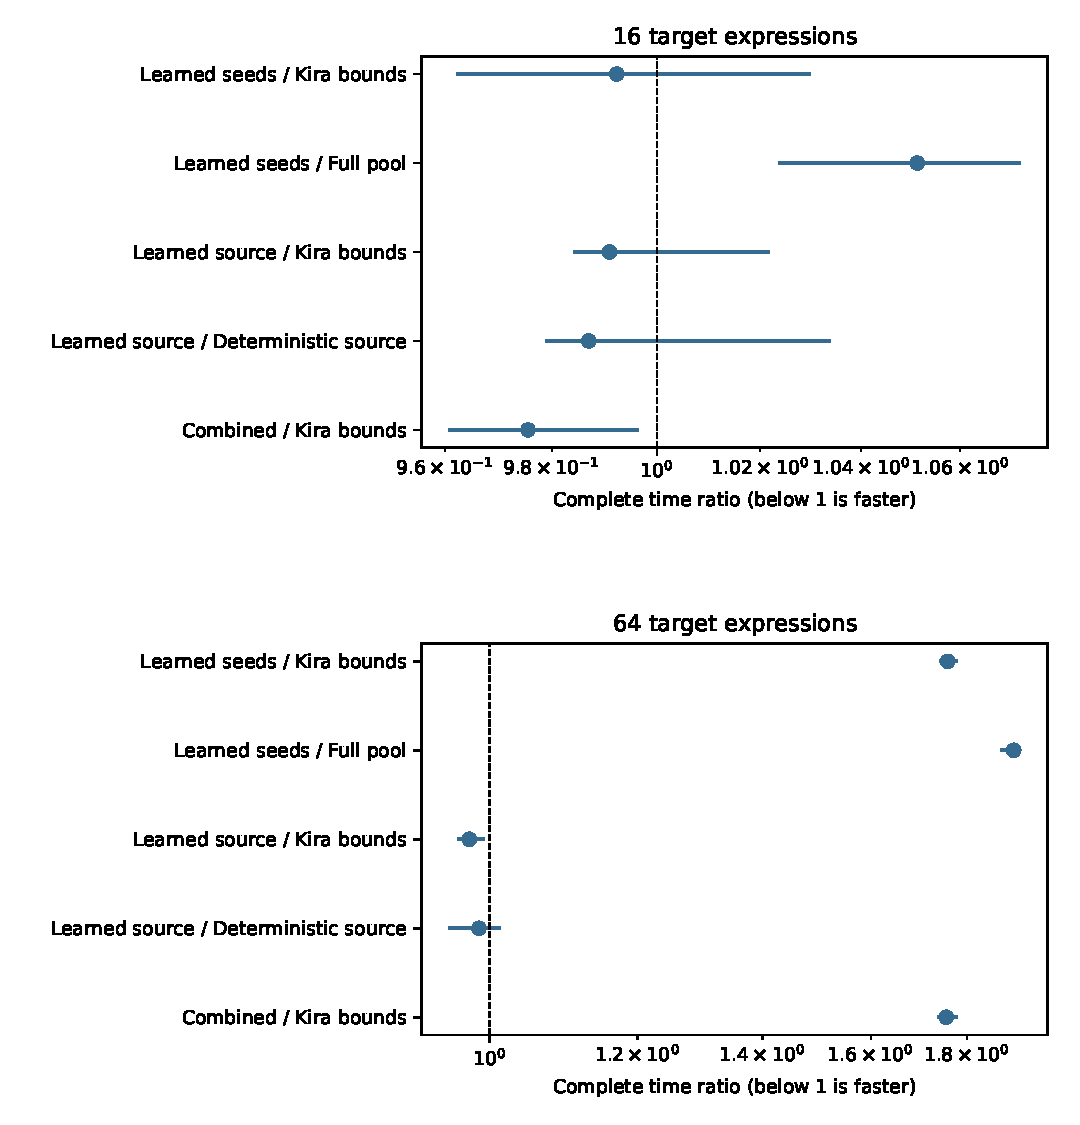
\includegraphics[width=\textwidth]{figures/native_transfer_times.pdf}
 \caption{Complete-time ratios in the two-loop transfer comparison for
 16 targets (upper panel) and 64 targets (lower panel). Points show
 ratios of five-repeat medians, and bars show descriptive paired-repeat
 intervals. All times include prediction, target preparation, exact
 reduction, combination, checks and any required fallback.}
 \label{fig:native-transfer}
\end{figure}
